\documentclass[a4paper]{article}

  \usepackage{fullpage} % Package to use full page
  \usepackage{parskip} % Package to tweak paragraph skipping
  \usepackage{tikz} % Package for drawing
  \usepackage{tkz-graph}
  \usepackage{amsmath}
  \usepackage{siunitx} % Package for scientific units
  \usepackage{amsfonts}
  \usepackage{amssymb}
  \usepackage{hyperref}
  \usepackage[utf8]{inputenc}
  \usepackage[english]{babel}
  \usepackage{multicol}
  \usepackage{graphicx} % Package for including images
  \graphicspath{ {./images/} }
  
  \DeclareUnicodeCharacter{2212}{-}
  \newcommand\tab[1][0.5cm]{\hspace*{#1}}
  
  \title{Homework 4}
  \author{Adrian Darian}
  \date{12/4/2020}
  
  \begin{document}
  
\maketitle
  
\section*{Chapter 5}
\begin{itemize}
	\item[22] Explain why TIME\_WAIT is a somewhat more serious problem if the server initiates the close than if the client does. Describe a situation in which this might reasonably happen. \\
	      \textbf{Answer:} Since clients handle a lot more connectons at once it is crucial to uphold a form of TIME\_WAIT so that the server may handle all incoming and outgoing endpoints.
	\item[25] Suppose a TCP connection, with window size 1, loses every other packet. Those that do arrive have RTT= 1 second. What happens? What happens to TimeOut? Do this for two cases: \\
	      \begin{itemize}
	      	\item[(a)] After a packet is eventually received, we pick up where we left off, resuming with Estimated RTT initialized to its pre-timeout value, and TimeOut double that. \\
	      	      \textbf{Answer:} The TimeOut does not change due to the fact that our RTT becomes two times that of our EstimatedRTT and will resume once it is received.
	      	\item[(b)] After a packet is eventually received, we resume with TimeOut initialized to the last exponentially backed-off value used forthe timeout interval. \\
	      	      \textbf{Answer:} The TimeOut will eventually double because we would need to apply a back-off time.
	      \end{itemize} 
	      In the following four exercises, the calculations involved are straight forward with a spreadsheet. 
	\item[26] Suppose, in TCP’s adaptive retransmission mechanism, that Estimated RTT is 4.0 seconds at some point and subsequent measured RTT’s all are 1.0 second. How long does it take before the TimeOut value, as calculated by the Jacobson/Karels algorithm, falls below 4.0 seconds? Assume a plausible initialvalue of Deviation; how sensitive is your answer to this choice? Use $\si{\delta}$ = 1/8 \\
	      \textbf{Answer:}
	      \begin{tabular}{cccccc}
	      	Iteration & SampleRTT & EstimationRTT & Deviation & difference & TimeOut \\
	      	0         & 1.00      & 4.00          & 1.00      &            &         \\
	      	1         & 1.00      & 3.63          & 1.25      & -3.00      & 8.63    \\
	      	2         & 1.00      & 3.31          & 1.42      & -2.63      & 8.99    \\ 
	      	3         & 1.00      & 3.03          & 1.53      & -2.31      & 9.15    \\
	      	4         & 1.00      & 2.78          & 1.59      & -2.03      & 9.14    \\
	      	5         & 1.00      & 2.56          & 1.61      & -1.78      & 9.00    \\ 
	      	6         & 1.00      & 2.37          & 1.61      & -1.56      & 8.81    \\
	      	7         & 1.00      & 2.20          & 1.58      & -1.37      & 8.52    \\
	      	8         & 1.00      & 2.05          & 1.54      & -1.20      & 8.21    \\
	      	9         & 1.00      & 1.92          & 1.48      & -1.05      & 7.84    \\
	      	10        & 1.00      & 1.81          & 1.41      & -.92       & 7.45    \\
	      	11        & 1.00      & 1.71          & 1.34      & -.81       & 7.07    \\
	      	12        & 1.00      & 1.63          & 1.27      & -.71       & 6.71    \\
	      	13        & 1.00      & 1.56          & 1.19      & -.63       & 6.32    \\
	      	14        & 1.00      & 1.49          & 1.12      & -.56       & 5.97    \\
	      	15        & 1.00      & 1.43          & 1.05      & -.49       & 5.63    \\
	      	16        & 1.00      & 1.38          & .98       & -.43       & 5.30    \\
	      	17        & 1.00      & 1.34          & .91       & -.38       & 4.98    \\
	      	18        & 1.00      & 1.30          & .84       & -.34       & 4.66    \\
	      	19        & 1.00      & 1.27          & .78       & -.30       & 4.39    \\
	      	20        & 1.00      & 1.24          & .72       & -.27       & 4.12    \\
	      	21        & 1.00      & 1.21          & .66       & -.24       & 3.85    \\
	      \end{tabular} 
	\item[29] Suppose that TCP is measuring RTTs of 1.0 second, with a mean deviation of 0.1 second. Suddenly the RTT jumps to 5.0 seconds, with no deviation. Compare the behaviors of the original and Jacobson/Karels algorithms for computing TimeOut. Specifically, how many timeouts are encountered with each algorithm? Whatis the largest TimeOut calculated? Use $\si{\delta}$= 1/8. \\
	      \textbf{Answer:} \\
	      \begin{tabular}{ccccccc}
	      	  &           &               &           &            & new TimeOut               & old TimeOut     \\
	      	  & SampleRTT & EstimationRTT & Deviation & difference & EstimationRTT+4xDeviation & 2xEstimationRTT \\
	      	  &           &               & 1.00      & 0.10       & 1.40                      & 2.00            \\
	      	1 & 5.00      & 1.50          & 0.59      & 4.00       & 3.85                      & 3.00            \\
	      	2 & 5.00      & 1.94          & 0.95      & 3.50       & 5.74                      & 3.88            \\
	      	3 & 5.00      & 2.32          & 1.22      & 3.06       & 7.18                      & 4.64            \\
	      	4 & 5.00      & 2.66          & 1.40      & 2.68       & 8.25                      & 5.32            \\
	      \end{tabular}
\end{itemize}

\section*{Chapter 6}
\begin{itemize}
	\item[16] Assume that TCP implements an extension that allows window sizes much larger than 64 KB. Suppose that you are using this extended TCP over a 1-Gbps link with a latency of 50 ms totransfer a 10-MB file, and the TCP receive window is 1 MB. If TCP sends 1-KB packets (assuming no congestion and no lostpackets): \\
	      \begin{itemize}
	      	\item[(a)] How many RTTs does it take until slow start opens the send window to 1 MB? \\
	      	      \textbf{Answer:} $2^{10}$KB
	      	\item[(b)] How many RTTs does it take to send the file? \\
	      	      \textbf{Answer:} 14 RTTs
	      	\item[(c)] If the time to send the file is given by the number of required RTTs multiplied by the link latency, what is the effective through put for the transfer? What percentage of the link bandwidth is utilized? \\
	      	      \textbf{Answer:} 114.3 Mbps which is 11.4\% of the bandwidth
	      \end{itemize} 
	\item[17] Consider a simple congestion-control algorithm that uses linear increase and multiplicative decrease but not slow start, that works in units of packets rather than bytes, and that starts each connection with a congestion window equal to one packet. Give a detailed sketch of this algorithm. Assume the delay is latency only and that when a group of packets is sent only a single ACK is returned. Plot the congestion window as a function of round-trip times for the situation in which the following packets are lost: 9,25, 30, 38, and 50. For simplicity, assume a perfect timeout mechanism that detects a lost packet exactly 1 RTT after it is transmitted. \\
		  \textbf{Answer:} With the window size of the sender beginning at a single packet. Then we increase that window size proportionally over time and our RTT allows us to forgo any packets being processed. \\
		  \begin{tabular}{cccccc}
			  RTT & 5 & 6 & 7 & 8 & 9 \\
			  Sent Packets & 9-10 & 11-13 & 14-17 & 18-22 & 23-28 \\
		  \end{tabular} 
	\item[23] Suppose the R–B link in the previous exercise changes from a bandwidth delay to a propagation delay, so that two packets now take 1 second to send. List what is sent and received during the first 8 seconds. Assume a static timeout value of 2 seconds, thats low start is used on a timeout, and that ACKs sent at about the same time are consolidated. Note that R’s queue size is now irrelevant (why?). \\
	      \textbf{Answer:} 
	      \begin{tabular}{cccc}
	      	    & A recvs & cwnd & A sends data \# \\
	      	T=0 &         & 1    & 1               \\
	      	T=1 & Ack1    & 2    & 2,3             \\
	      	T=2 & Ack3    & 4    & 4,5,6,7         \\
	      	T=3 & Ack7    & 8    & 8–15          \\
	      	T=4 & Ack15   & 16   & 16–31         \\
	      	T=5 & Ack31   & 32   & 32–63         \\
	      	T=6 & Ack63   & 64 6 & 4–127         \\
	      	T=7 & Ack127  & 128  & 127–255       \\
	      	T=8 & Ack255  & 256  & 255–511       \\
	      \end{tabular}
	\item[27] Consider the TCP trace in Figure 6.28. Identify time intervals representing slow start on startup, slow start after timeout, and linear-increase congestion avoidance. Explain what is going on from T= 0.5 to T= 1.9. The TCP version that generated this trace includes a feature absent from the TCP that generated Figure 6.11. What is this feature? This trace and the one in Figure 6.13 both lack a feature. What is it? \\
	      \textbf{Answer:} 
	\item[28] Suppose you are downloading a large file over a 3-KBps phonelink. Your software displays an average-bytes-per-second counter. How will TCP congestion control and occasional packet losses cause this counter to fluctuate? Assume that only a third, say, of the total RTT is spent on the phone link. \\
	      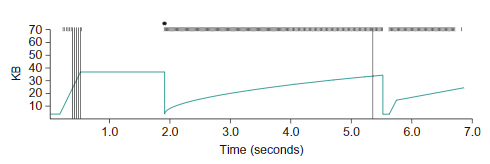
\includegraphics[scale=0.5]{6-28.png} \\
	      \textbf{Answer:} 3/6 -> 6/9 -> 9/12 = 1 - 1/N
	\item[31] Suppose a TCP connection has a window size of eight segmentsand an RTT of 800 ms, the sender sends segments at a regular rateof one every 100 ms, and the receiver sends ACKs back at the same rate without delay. A segment is lost, and the loss is detected by the fast retransmit algorithm on the receipt of the third duplicate ACK. At the point when the ACK of there transmitted segment finally arrives, how much total time has the sender lost (compared to loss less transmission) if \\
	      \begin{itemize}
	      	\item[(a)] The sender waits for the ACK from the retransmitted lost packet before sliding the window forward again? \\
	      	      \textbf{Answer:} 1/3 of the time is put towards detecting an ACK and 2/3 of the time is the RTT waiting for an ACK. Leaving T=-800 and lost ACK T=0
	      	\item[(b)] The sender uses the continued arrival of each duplicate ACK as an indication it may slide the window forward one segment? \\
	      	      \textbf{Answer:} 700ms with 4 extra chances to transmit data
	      \end{itemize}
\end{itemize}

\section*{Chapter 9}
\begin{itemize}
	\item[10] In HTTP version 1.0, a server marked the end of a transfer by closing the connection. Explain why, in terms of the TCP layer, this was a problem for servers. Find out how HTTP version 1.1 avoids this. How might a general-purpose request/reply protocol address this? \\
	      \textbf{Answer:} Closing a server requires extra records to be recorded while the TIME\_WAIT state is processed. After the HTTP 1.1 the server can transfer all request/reply protocol may be addressed.  
	\item[14] Suppose a very large website wants a mechanism by which clients access whichever of multiple HTTP servers is “closest” by some suitable measure.
	      \begin{itemize}
	      	\item[(a)] Discuss developing a mechanism within HTTP for doing this. \\
	      	      \textbf{Answer:} The communication between the client and a server would allow the client to request alternate servers from said server when possible.
	      	\item[(b)] Discuss developing a mechanism within DNS for doing this. Compare the two. Can either approach be made to work without upgrading the browser? \\
	      	      \textbf{Answer:} From responses coming back from the servers the client catalogs all possible connections (alternates) and prceeds to determine which one to establish a connection to based on the RTT
	      \end{itemize}
	\item[22] ARP and DNS both depend on caches; ARP cache entry life times are typically 10 minutes, while DNS cache life times are on the order of days. Justify this difference. What undesirable consequences might there be in having too long a DNS cacheentry lifetime? \\
	      \textbf{Answer:} For starters ARP is always local while DNS is considered the opposite. ARP is primarily used for a very small area while DNS is used more for a much broader and larger area. 
	\item[38] What problem would a DNS-based redirection mechanism encounter if it wants to select an appropriate server based on current load information? \\
	      \textbf{Answer:} A problem lies in the caching of the DNS responses and how it would require more small packets to be sent which intune relays more querying of the DNS servers.
\end{itemize}

\end{document}